% ------------------------------------------------------------------------
% ------------------------------------------------------------------------
% Modelo de TCC do curso de Engenharia de Controle e Automação - UFSC/Campus Blumenau
% Autor: Ciro André Pitz
% Revisão: Brenda Teresa Porto de Matos
% O presente modelo foi obtido a partir do modelo desenvolvido por Alisson Lopes Furlani disponível na BU/UFSC.
% ------------------------------------------------------------------------
% ------------------------------------------------------------------------

\documentclass[
12pt,				% tamanho da fonte
%openright,			% capítulos começam em pág ímpar (insere página vazia caso preciso)
oneside,			% para impressão no anverso. Oposto a twoside
a4paper,			% tamanho do papel. 
chapter=TITLE,		% títulos de capítulos convertidos em letras maiúsculas
section=TITLE,		% títulos de seções convertidos em letras maiúsculas
%subsection=TITLE,	% títulos de subseções convertidos em letras maiúsculas
%subsubsection=TITLE,% títulos de subsubseções convertidos em letras maiúsculas
% -- opções do pacote babel --
english,			% idioma adicional para hifenização
brazil				% o último idioma é o principal do documento
]{abntex2}

\usepackage{configs/eca_ufsc_bnu} % personalização da ABNTEX2 
\addbibresource{pos_textual/referencias.bib} % Seus arquivos de referências

%---------------------------------------------------------------------------------------------
%--------- DADOS BÁSICOS DO TCC (Preencher todos) -------------------------------------
%---------------------------------------------------------------------------------------------
%Substituir 'Nome completo do autor' pelo seu nome.
\autor{Nome completo do autor(a)}
% FIXME Substituir 'Título do trabalho' pelo título da trabalho.
\titulo{Título do trabalho}
% Substituir 'Subtítulo (se houver)' pelo subtítulo da trabalho. 
% Se não houver subtítulo, basta deletar o texto.
\subtitulo{subtítulo (se houver)}

\orientador{Prof. Nome, Dr.}
% Se for orientado por uma mulher, comente a linha acima e descomente a linha a seguir.
% \orientador[Orientadora]{Profa. Nome, Dra.}

% Caso não tenha coorientador, comente a linha a seguir.
\coorientador{Prof. Nome, Dr.}
% Se for coorientado por uma mulher, comente a linha acima e descomente a linha a seguir.
% \coorientador[Coorientadora]{Profa. Nome, Dra.}

\dia{dia}
\mes{mês}
\ano{ano}
\local{Blumenau}
\formacao{Engenheiro de Controle e Automação}
% Se for mulher, comente a linha acima e descomente a linha a seguir.
%\formacao{Engenheira de Controle e Automação}

\bancanomea{Prof. Nome, Dr.} %Primeiro membro da banca (normalmente o orientador). Altere as abreviações para o feminino (exemplo: Profa., Dra.) quando for o caso.
\bancainsta{Nome da instituição ou empresa} %Nome da instituição (UFSC, por exemplo) ou empresa do primeiro membro da banca

\bancanomeb{Prof. Nome, Dr.} %Segundo membro da banca. Altere as abreviações para o feminino (exemplo: Profa., Dra.) quando for o caso.
\bancainstb{Nome da instituição ou empresa} %Nome da instituição (UFSC, por exemplo) ou empresa do segundo membro da banca

\bancanomec{Prof. Nome, Dr.} %Terceiro membro da banca. Altere as abreviações para o feminino (exemplo: Profa., Dra.) quando for o caso.
\bancainstc{Nome da instituição ou empresa} %Nome da instituição (UFSC, por exemplo) ou empresa do terceiro membro da banca

%Resumo e palavras-chave do trabalho
\resumotcc{No resumo são ressaltados o objetivo da pesquisa, o método utilizado, as discussões e os resultados com destaque apenas para os pontos principais. O resumo deve ser significativo, composto de uma sequência de frases concisas, afirmativas, e não de uma enumeração de tópicos. Não deve conter citações. Deve usar o verbo na voz ativa e na terceira pessoa do singular. O texto do resumo deve ser digitado, em um único bloco, sem espaço de parágrafo. O espaçamento entre linhas é simples e o tamanho da fonte é 12. Abaixo do resumo, informar as palavras-chave (palavras ou expressões significativas retiradas do texto) ou, termos retirados de thesaurus da área. Deve conter de 150 a 500 palavras. O resumo é elaborado de acordo com a NBR 6028.}
\palavraschave{palavra-chave 1; palavra-chave 2; palavra-chave 3.}

%Abstract e keywords do trabalho
\abstracttcc{Resumo traduzido para outros idiomas, neste caso, inglês. Segue o formato do resumo feito na língua vernácula. As palavras-chave traduzidas, versão em língua estrangeira, são colocadas abaixo do texto precedidas pela expressão ``Keywords'', separadas por ponto e vírgula.}
\keywords{keyword 1; keyword 2; keyword 3.}

%Agradecimentos (opcional). Caso não queira inserir, deixe em branco (\agradecimentostcc{} )
\agradecimentostcc{Inserir os agradecimentos aos colaboradores à execução do trabalho.}

%Epígrafe (opcional). Caso não queira inserir, deixe em branco (\epigrafetcc{} )
\epigrafetcc{Texto da Epígrafe. Citação relativa ao tema do trabalho. É opcional. A epígrafe pode também aparecer na abertura de cada seção ou capítulo. Deve ser elaborada de acordo com a NBR 10520. (SOBRENOME do autor da epígrafe, ano)}

%Decatória (opcional). Caso não queira inserir, deixe em branco (\dedicatoriatcc{} )
\dedicatoriatcc{Este trabalho é dedicado aos meus colegas de classe e aos meus queridos pais.}

%Lista de quadros
%Além de figuras e tabelas, o TCC contém quadros? Caso afirmativo digite sim ou deixe em branco para não (\contemquadros{}).
\contemquadros{sim}

%Lista de siglas (opcional).
%Deseja incluir lista de abreviaturas e siglas? Caso afirmativo digite sim ou deixe em branco para não (\contemsiglas{}).
\contemsiglas{sim}

%Lista de símbolos (opcional).
%Deseja incluir lista de símbolos? Caso afirmativo digite sim ou deixe em branco para não (\contemsimbolos{}).
\contemsimbolos{sim}

%-------------------------FIM DOS DADOS BÁSICOS DO TCC--------------------------------------------




% ajusta espaçamento das listas itemize e enumerate
\setitemize{topsep=0pt,itemsep=0pt,leftmargin=\parindent+\labelwidth-\labelsep}
\setenumerate{topsep=0pt,itemsep=0pt,leftmargin=\parindent+\labelwidth-\labelsep}

% define a macro \Autoref to allow multiple references to be passed to \autoref
\makeatletter
\newcommand\Autoref[1]{\@first@ref#1,@}
\def\@throw@dot#1.#2@{#1}% discard everything after the dot
\def\@set@refname#1{%    % set \@refname to autoefname+s using \getrefbykeydefault
	\edef\@tmp{\getrefbykeydefault{#1}{anchor}{}}%
	\xdef\@tmp{\expandafter\@throw@dot\@tmp.@}%
	\ltx@IfUndefined{\@tmp autorefnameplural}%
	{\def\@refname{\@nameuse{\@tmp autorefname}s}}%
	{\def\@refname{\@nameuse{\@tmp autorefnameplural}}}%
}
\def\@first@ref#1,#2{%
	\ifx#2@\autoref{#1}\let\@nextref\@gobble% only one ref, revert to normal \autoref
	\else%
	\@set@refname{#1}%  set \@refname to autoref name
	\@refname~\ref{#1}% add autoefname and first reference
	\let\@nextref\@next@ref% push processing to \@next@ref
	\fi%
	\@nextref#2%
}
\def\@next@ref#1,#2{%
	\ifx#2@ e~\ref{#1}\let\@nextref\@gobble% at end: print e+\ref and stop
	\else, \ref{#1}% print  ,+\ref and continue
	\fi%
	\@nextref#2%
}
\makeatother

% Cria comando para referenciar Anexo automaticamente \refanexo
\newcommand{\refanexo}[1]{\hyperref[#1]{Anexo~\ref{#1}}}

% Define comandos para tabelas que permite ajustar o tamanho da coluna e manter alinhamento C, R ou L
%\newcommand{\PreserveBackslash}[1]{\let\temp=\\#1\let\\=\temp}
\newcolumntype{C}[1]{>{\centering\let\arraybackslash}m{#1}}
\newcolumntype{R}[1]{>{\RaggedLeft\let\arraybackslash}m{#1}}
\newcolumntype{L}[1]{>{\RaggedRight\let\arraybackslash}m{#1}}


% ---
% Filtering and Mapping Bibliographies
% ---
\DeclareSourcemap{
	\maps[datatype=bibtex]{
		% remove fields that are always useless
		\map{
			\step[fieldset=abstract, null]
			\step[fieldset=pagetotal, null]
			\step[fieldset=doi, null]
		}
		% remove URLs for types that are primarily printed
		\map{
			\pernottype{software}
			\pernottype{online}
			\pernottype{report}
			\pernottype{techreport}
			\pernottype{standard}
			\pernottype{manual}
			\pernottype{misc}
			\step[fieldset=url, null]
			\step[fieldset=urldate, null]
		}
		\map{
			\pertype{inproceedings}
			% remove mostly redundant conference information
			%\step[fieldset=venue, null]
			%\step[fieldset=eventdate, null]
			%\step[fieldset=eventtitle, null]
			% do not show ISBN for proceedings
			\step[fieldset=isbn, null]
			% Citavi bug
			%\step[fieldset=volume, null]
		}
	}
}
% ---

\preambulo
{%
	Trabalho de Conclusão de Curso de Graduação em Engenharia de Controle e Automação do Centro Tecnológico, de Ciências Exatas e Educação da Universidade Federal de Santa Catarina como requisito para a obtenção~do~título~de~\imprimirformacao.
}
% ---

% ---
% Configurações de aparência do PDF final
% ---
% alterando o aspecto da cor azul
\definecolor{blue}{RGB}{41,5,195}
% informações do PDF
\makeatletter
\hypersetup{
	%pagebackref=true,
	pdftitle={\@title}, 
	pdfauthor={\@author},
	pdfsubject={\imprimirpreambulo},
	pdfcreator={LaTeX with abnTeX2},
	pdfkeywords={ufsc, latex, abntex2}, 
	colorlinks=true,       		% false: boxed links; true: colored links
	linkcolor=black,%blue,          	% color of internal links
	citecolor=black,%blue,        		% color of links to bibliography
	filecolor=black,%magenta,      		% color of file links
	urlcolor=blue,
	bookmarksdepth=4
}
\makeatother
% ---

% Definição das siglas e símbolos

%----------------- LISTA DE ABREVIATURAS E SIGLAS--------------------------------------
\siglalista{ABNT}{Associação Brasileira de Normas Técnicas}

%Para usar uma dada sigla ABC ao longo do texto, use \acrfull{ABC} se quiser apresentar a sigla e sua definição.
%Se quiser apresentar apenas a sigla, use \acrshort{ABC}.






%-----------------SÍMBOLOS---------------------------------------------------------------
\simbololista{C}{\ensuremath{C}}{Circunferência de um círculo}
\simbololista{pi}{\ensuremath{\pi}}{Número pi} 
\simbololista{r}{\ensuremath{r}}{Raio de um círculo}
\simbololista{A}{\ensuremath{A}}{Área de um círculo}

%Para usar um dado símbolo SIMB ao longo do texto, use \gls{SIMB}.

% compila a lista de abreviaturas e siglas e a lista de símbolos
\makenoidxglossaries 

% compila o indice
\makeindex


% ------------------------------------------------------------------------------------------------
% --------------------------INÍCIO DO DOCUMENTO---------------------------------------------
% ------------------------------------------------------------------------------------------------
\begin{document}
	
	% Seleciona o idioma do documento (conforme pacotes do babel)
	%\selectlanguage{english}
	\selectlanguage{brazil}
	
	% Retira espaço extra obsoleto entre as frases.
	\frenchspacing 
	
	% Espaçamento 1.5 entre linhas
	\OnehalfSpacing
	
	% Corrige justificação
	%\sloppy
	

	%Elementos pré-textuais
	% \pretextual %a macro \pretextual é acionado automaticamente no início de \begin{document}
	% Capa, folha de rosto, ficha bibliografica, errata, folha de aprovação
	% Dedicatória, agradecimentos, epígrafe (opcional), resumos, listas
	% Capa
\imprimircapa


% Folha de rosto
% o * indica que haverá a ficha bibliográfica
\imprimirfolhaderosto*

% Inserir a ficha bibliografica
% http://ficha.bu.ufsc.br/
\begin{fichacatalografica}
	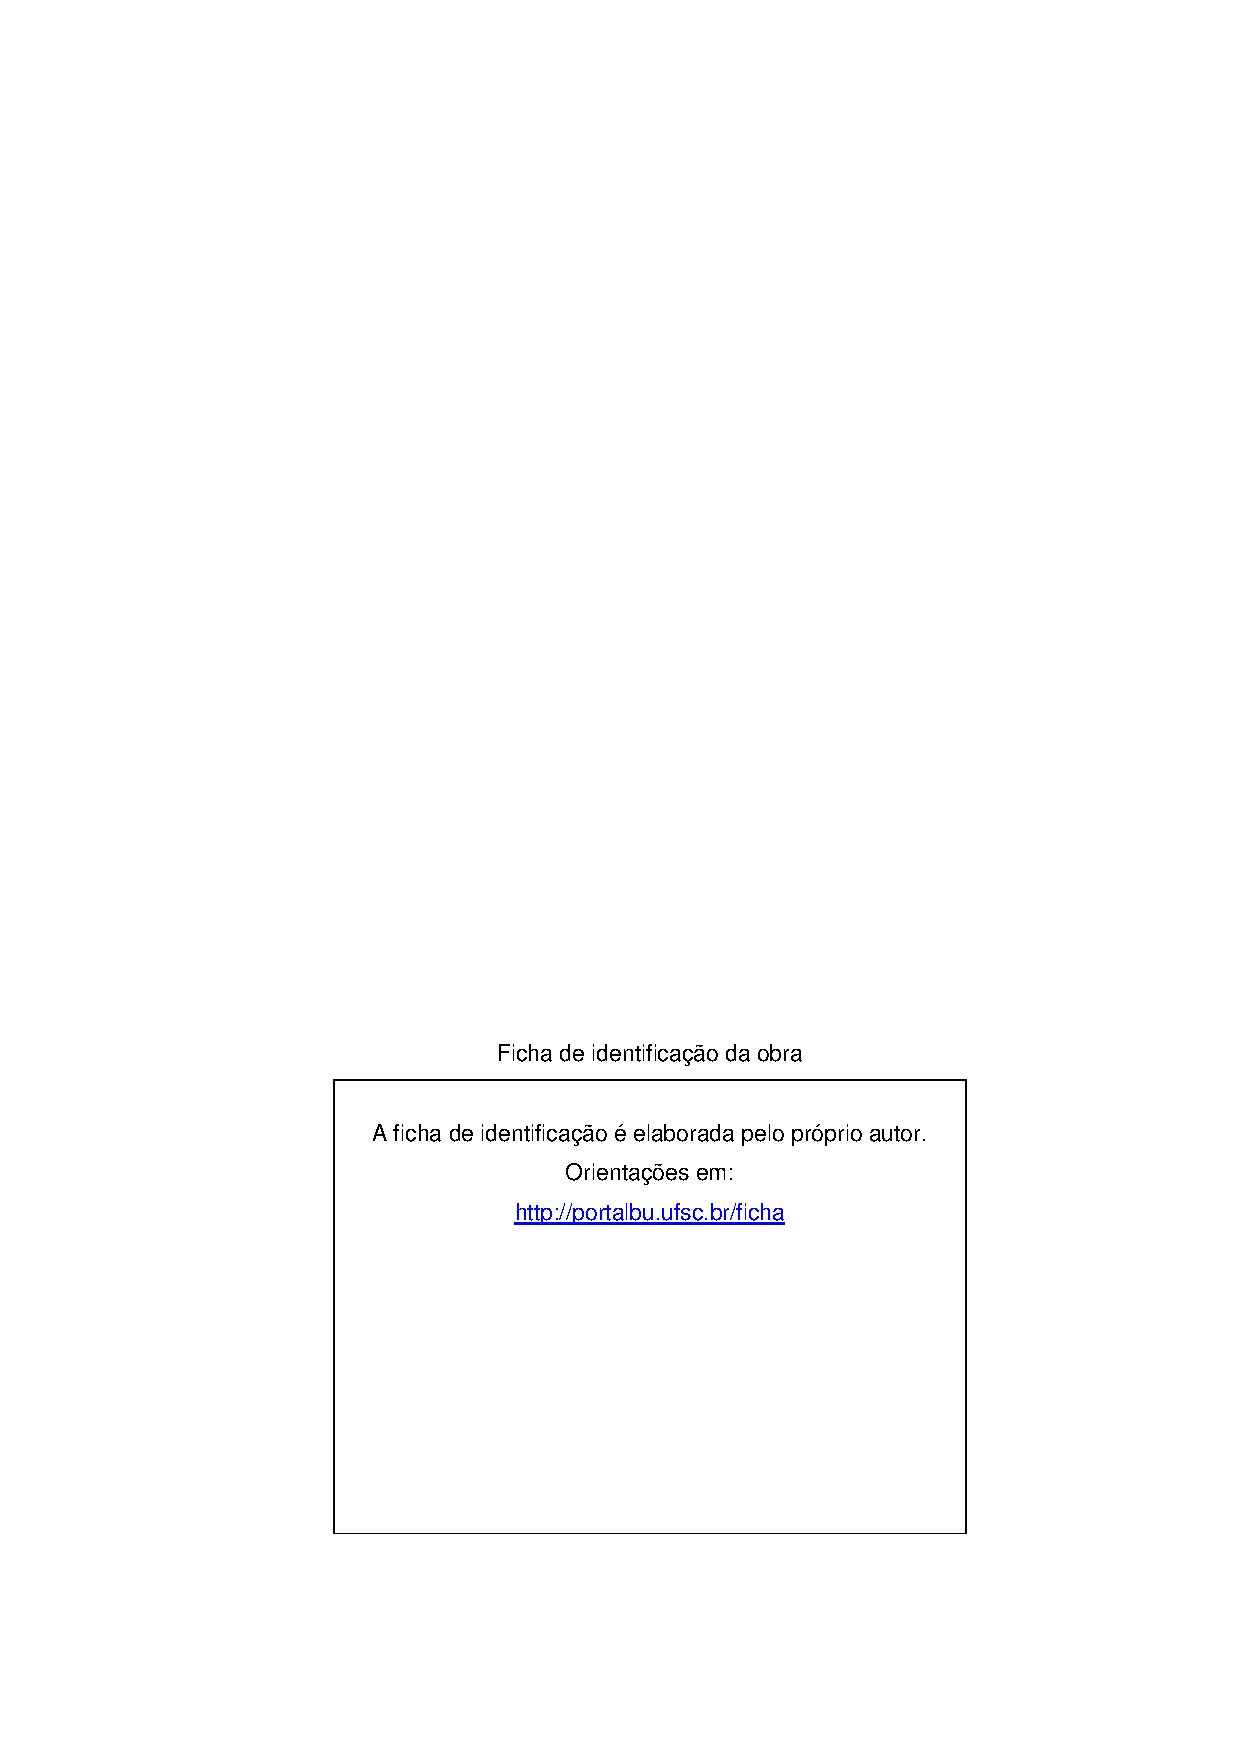
\includepdf{pre_textual/ficha_catalografica.pdf}
\end{fichacatalografica}

% Inserir folha de aprovação
\begin{folhadeaprovacao}
	\OnehalfSpacing
	\centering
	\imprimirautor\\%
	\vspace{24pt}		
	\textbf{\imprimirtitulo}%
	\ifnotempty{\imprimirsubtitulo}{:~\imprimirsubtitulo}\\%
	%		\vspace*{31.5pt}%3\baselineskip
	\vspace*{\baselineskip}
	%\begin{minipage}{\textwidth}
	Este Trabalho de Conclusão de Curso foi julgado adequado para obtenção do Título de ``\imprimirformacao'' e aprovado em sua forma final pelo Curso de Graduação em Engenharia de Controle e Automação.\\
	\vspace{12pt}
	\imprimirlocal, \imprimirdia~de~\imprimirmes~de~\imprimirano.\\
	
	\vspace*{18pt}
	\textbf{Banca Examinadora:}\\
	
	\vspace*{24pt}
	\assinatura{\OnehalfSpacing \imprimirbancanomea}
	\vspace{6pt}
	\imprimirbancainsta\\
	
	\vspace*{24pt}
	\assinatura{\OnehalfSpacing \imprimirbancanomeb}
	\vspace{6pt}
	\imprimirbancainstb\\
	
	\vspace*{24pt}
	\assinatura{\OnehalfSpacing \imprimirbancanomec}
	\vspace{6pt}
	\imprimirbancainstc\\
	
\end{folhadeaprovacao}

% Dedicatória
\ifnotempty{\imprimirdedicatoriatcc}{
\begin{dedicatoria}
	\vspace*{\fill}
	\noindent
	\begin{adjustwidth*}{}{7.5cm} 
		\textit{\imprimirdedicatoriatcc}
	\end{adjustwidth*}
\end{dedicatoria}
}

% Agradecimentos
\ifnotempty{\imprimiragradecimentostcc}{
\begin{agradecimentos}
	\imprimiragradecimentostcc
\end{agradecimentos}
}

% Epígrafe
\ifnotempty{\imprimirepigrafetcc}{
\begin{epigrafe}
	\vspace*{\fill}
        \noindent
	\begin{adjustwidth*}{}{7.5cm}
	       \textit{\imprimirepigrafetcc}
        \end{adjustwidth*}
\end{epigrafe}
}


% Resumo
\setlength{\absparsep}{18pt} % ajusta o espaçamento dos parágrafos do resumo
\begin{resumo}
	\SingleSpacing
	\imprimirresumotcc
	
	\textbf{Palavras-chave}: \imprimirpalavraschave
\end{resumo}

% Abstract
\begin{resumo}[Abstract]
	\SingleSpacing
	\imprimirabstracttcc
		
	\textbf{Keywords}: \imprimirkeywords
\end{resumo}


{%hidelinks
	\hypersetup{hidelinks}
	
	% inserir lista de figuras
	\pdfbookmark[0]{\listfigurename}{lof}
	\listoffigures*
	\cleardoublepage
	
	% inserir lista de quadros
	\ifnotempty{\verificaquadros}{
		\pdfbookmark[0]{\listofquadrosname}{loq}
		\listofquadros*
		\cleardoublepage
	}
	
	% inserir lista de tabelas
	\pdfbookmark[0]{\listtablename}{lot}
	\listoftables*
	\cleardoublepage
	
	% inserir lista de abreviaturas e siglas (devem ser declarados no preambulo)
	\ifnotempty{\verificasiglas}{
	\imprimirlistadesiglas
	}
	
	% inserir lista de símbolos (devem ser declarados no preambulo)
	\ifnotempty{\verificasimbolos}{
	\imprimirlistadesimbolos
	}
	
	% inserir o sumario
	\pdfbookmark[0]{\contentsname}{toc}
	\tableofcontents*
	\cleardoublepage
	
}%hidelinks

	% Elementos textuais
	\textual
	
	% 1 - Introdução
	% ----------------------------------------------------------
\chapter{Introdução}
% ----------------------------------------------------------

As orientações aqui apresentadas são baseadas em um conjunto de normas elaboradas pela \glsxtrfull{ABNT}. Além das normas técnicas, a Biblioteca também elaborou uma série de tutoriais, guias, \textit{templates} os quais estão disponíveis em seu site, no endereço \url{http://portal.bu.ufsc.br/normalizacao/}.

Paralelamente ao uso deste \textit{template} recomenda-se que seja utilizado o \textbf{Tutorial de Trabalhos Acadêmicos} (disponível neste link \url{https://repositorio.ufsc.br/handle/123456789/180829}) e/ou que o discente \textbf{participe das capacitações oferecidas da Biblioteca Universitária da UFSC}.

Este \textit{template} está configurado apenas para a impressão utilizando o anverso das folhas, caso você queira imprimir usando a frente e o verso, acrescente a opção \textit{openright} e mude de \textit{oneside} para \textit{twoside} nas configurações da classe \textit{abntex2} no início do arquivo principal \textit{main.tex} \cite{abntex2classe}.

Os trabalhos de conclusão de curso (TCC) de graduação e de especialização não são entregues em formato impresso na Biblioteca Universitária. Porém, sua versão PDF deve ser disponibilizada no Repositório Institucional. Consulte as orientações disponibilizadas no Moodle da disciplina de TCC sobre os procedimentos adotados para a entrega.

\section{Recomendações de uso}
Este \textit{template} foi elaborado em \LaTeX. O sumário é gerado automaticamente de acordo com a norma NBR 6027/2012 utilizando a sequência abaixo para diferenciação gráfica nas divisões de seção e subseção.

\vspace{12pt}

\textbf{1 SEÇÃO PRIMÁRIA}

1.1 SEÇÃO SECUNDÁRIA

\textbf{1.1.1 Seção terciária}

\textit{1.1.1.1 Seção quartenária}

1.1.1.1.1 Seção quinária

\vspace{12pt}

\begin{alineas}
    \item Seção primária, use o comando \verb|\section{}|.
    \item Seção secundária, use o comando \verb|\subsection{}|.
    \item Seção terciária, use o comando \verb|\subsubsection{}|.
    \item Seção quartenária, use o comando \verb|\subsubsubsection{}|.
    \item Seção quinária, use o comando \verb|\subsubsubsubsection{}|.
    \item Título das seções de referências, apêndice e anexo são gerados automaticamente pelo \textit{template}.
    \item Para citação com mais de três linhas use o comando \verb|\begin{citacao}|.
    \item Note de rodapé, use o comando \verb|\footnote{}|\footnote{A nota de rodapé é automaticamente formatada pelo \textit{template}.}
\end{alineas}

\section{Objetivos}


Nas seções abaixo estão descritos o objetivo geral e os objetivos específicos deste TCC.


\subsection{Objetivo Geral}


Descrição...


\subsection{Objetivos Específicos}


Descrição...
	
	% 2 - Desenvolvimento
	% ----------------------------------------------------------
\chapter{Desenvolvimento}\label{cap:desenvolvimento}
% ----------------------------------------------------------
Deve-se inserir texto entre as seções.

\section{Exposição do tema ou matéria}

É a parte principal e mais extensa do trabalho. Deve apresentar a fundamentação teórica, a metodologia, os resultados e a discussão. Divide-se em seções e subseções conforme a NBR 6024 \cite{NBR6024:2012}.

Quanto à sua estrutura e projeto gráfico, segue as recomendações da norma para preparação de trabalhos acadêmicos, a NBR 14724, de 2011 \cite{NBR14724:2011}.

\begin{figure}[htb]
	\caption{\label{fig:Fig_1}Elementos do trabalho acadêmico.}
	\begin{center}
		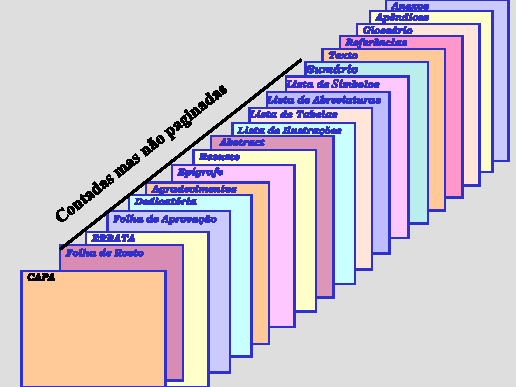
\includegraphics{figuras/imagem.pdf}
	\end{center}
	\fonte{Universidade Federal do Paraná (1996).}
\end{figure}

\subsection{Formatação do texto}

No que diz respeito à estrutura do trabalho, recomenda-se que:
\begin{alineas}
	\item o texto deve ser justificado, digitado em cor preta, podendo utilizar outras cores somente para as ilustrações;
	\item utilizar papel branco ou reciclado para impressão;
	\item \textbf{se o trabalho for impresso}, os elementos pré-textuais devem iniciar no anverso da folha, com exceção da ficha catalográfica ou ficha de identificação da obra;
	\item \textbf{se o trabalho for impresso}, os elementos textuais e pós-textuais devem ser digitados no anverso e verso das folhas;
	\item as seções primárias devem começar sempre em páginas ímpares, quando o trabalho for impresso e
	\item deixar um espaço entre o título da seção/subseção e o texto e entre o texto e o título da subseção.
\end{alineas}

No \autoref{qua:Quadro_1} estão as especificações para a formatação do texto.

\begin{quadro}[htb]
	\centering
	\caption{\label{qua:Quadro_1}Formatação do texto.}	
	\begin{tabular}{|l|p{11cm}|}
		\hline
		\textbf{Formato do papel} & A4.\\ \hline
		\textbf{Impressão}        & A norma recomenda que \textbf{caso seja necessário imprimir}, deve-se utilizar a frente e o verso da página.\\ \hline
		\textbf{Margens}          & Superior: 3, Inferior: 2, Interna: 3 e Externa: 2. Usar margens espelhadas quando o  trabalho for impresso.\\ \hline
		\textbf{Paginação}        & As páginas dos elementos pré-textuais devem ser contadas, mas não numeradas. Para trabalhos digitados somente no anverso, a numeração das páginas deve constar no canto superior direito da página, a 2 cm da borda, figurando a partir da primeira folha da  parte textual. Para trabalhos digitados no anverso e no verso, a numeração deve constar no canto superior direito, no anverso, e no canto superior esquerdo no verso.\\ \hline
		\textbf{Espaçamento}      & O texto deve ser redigido com espaçamento entre linhas 1,5, excetuando-se as citações de mais de três linhas, notas de rodapé, referências, legendas das ilustrações e das tabelas, natureza (tipo do trabalho, objetivo, nome da instituição a que é submetido e área de concentração), que devem ser digitados em espaço simples, com fonte menor. As referências devem ser separadas entre si por um espaço simples em branco.\\ \hline
		\textbf{Paginação}        & A contagem inicia na folha de rosto, mas se \textbf{insere o número da página na introdução} até o final do trabalho.\\ \hline
		\textbf{Fontes sugeridas} & Arial ou Times New Roman.\\ \hline
		\textbf{Tamanho da fonte} & \textbf{Fonte tamanho 12 para o texto}, incluindo os títulos das seções e subseções. As citações com mais de três linhas, notas de rodapé, paginação, dados internacionais de catalogação, legendas e fontes das ilustrações e das tabelas devem ser de tamanho menor. Adotamos, neste \textit{template} \textbf{fonte tamanho 10}.\\ \hline
		\textbf{Nota de rodapé}   & Devem ser digitadas dentro da margem, ficando separadas por um espaço simples por entre as linhas e por filete de 5 cm a partir da margem esquerda. A partir da segunda linha, devem ser alinhadas embaixo da primeira letra da primeira palavra da primeira linha.\\ \hline
	\end{tabular}
	\fonte{\textcite{NBR14724:2011}.}
\end{quadro}


\subsubsection{As ilustrações}

Independentemente do tipo de ilustração (quadro, desenho, figura, fotografia, mapa, entre outros), a sua identificação aparece na parte superior, precedida da palavra designativa. 

\begin{citacao}
	Após a ilustração, na parte inferior, indicar a fonte consultada (elemento obrigatório, mesmo que seja produção do próprio autor), legenda, notas e outras informações necessárias à sua compreensão (se houver). A ilustração deve ser citada no texto e inserida o mais próximo possível do texto a que se refere. \cite[p. 11]{NBR14724:2011}.
\end{citacao}

\subsubsection{Equações e fórmulas}

As equações e fórmulas devem ser destacadas no texto para facilitar a leitura.  Para numerá-las, usar algarismos arábicos entre parênteses e alinhados à direita. Pode-se adotar uma entrelinha maior do que a usada no texto \cite{NBR14724:2011}.

Por exemplo, a circunferência e a área de um círculo com raio $r$ são dados, respectivamente, por
\begin{equation}\label{eq:Eq_1}
\gls{C} = 2 \gls{pi} \gls{r}    %note que o comando \gls{} usa a definição da lista de símbolos. Se não houver lista de símbolos, a equação deve ser digitada normalmente, ou seja, C = 2 \pi r
\end{equation}
e
\begin{equation}\label{eq:Eq_2}
\gls{A} = \gls{pi} \gls{r}^2.
\end{equation}
É importante observar que a \autoref{eq:Eq_1} e a \autoref{eq:Eq_2} fazem parte da frase (note a letra ``e'' entre as equações e o ponto final após a \autoref{eq:Eq_2}). 

\subsubsubsection{Exemplo tabela}

De acordo com \textcite{ibge1993}, tabela é uma forma não discursiva de apresentar informações em que os números representam a informação central. Ver \autoref{tab:Tab_1}.

\begin{table}[htb]
	\ABNTEXfontereduzida
	\caption{\label{tab:Tab_1}Médias concentrações urbanas 2010-2011.}
	\begin{tabular}{@{}p{3.0cm}p{1.5cm}p{2cm}p{2.5cm}p{2.5cm}p{2.5cm}@{}}
		\toprule
		\textbf{Média concentração urbana} & \multicolumn{2}{l}{\textbf{População}} & \textbf{Produto Interno Bruto – PIB (bilhões R\$)} & \textbf{Número de empresas} & \textbf{Número de unidades locais} \\ \midrule
		\textbf{Nome}                      & \textbf{Total}   & \textbf{No Brasil}  &                                                   &                             & \\
		Ji-Paraná (RO)                     & 116 610          & 116 610             & 1,686                                             & 2 734                       & 3 082 \\
		Parintins (AM)                     & 102 033          & 102 033             & 0,675                                             & 634                         & 683 \\
		Boa Vista (RR)                     & 298 215          & 298 215             & 4,823                                             & 4 852                       & 5 187 \\
		Bragança (PA)                      & 113 227          & 113 227             & 0,452                                             & 654                         & 686 \\ \bottomrule
	\end{tabular}
	\fonte{\textcite{ibge2016}.}
\end{table}
	
	% 3 - Seção
	% ----------------------------------------------------------
\chapter{Seção}
% ----------------------------------------------------------

Este \textit{template} contém algumas seções criadas na tentativa de facilitar seu uso. No entanto, não há um limite máximo ou mínimo de seção a ser utilizado no trabalho. Cabe a cada autor definir a quantidade que melhor atenda à sua 
necessidade.  
	
	% 4 - Conclusão
	% ----------------------------------------------------------
\chapter{Conclusão}
% ----------------------------------------------------------

As conclusões devem responder às questões da pesquisa, em relação aos objetivos e às hipóteses. Devem ser breves, podendo apresentar recomendações e sugestões para trabalhos futuros.
	
	
	% Elementos pós-textuais
	\postextual
	
	
	% Referências bibliográficas
	\begingroup
	    \printbibliography[title=REFERÊNCIAS]
	\endgroup
	
	
	
	%Reconfiguração do título para apêndices e anexos
	 \renewcommand{\ABNTEXchapterupperifneeded}[1]{#1} 
	\makeatletter
	\settocpreprocessor{chapter}{%
      \let\tempf@rtoc\f@rtoc%
      \def\f@rtoc{%
      \texorpdfstring{{\tempf@rtoc}}{\tempf@rtoc}}%
      }
    \makeatother
	
	
	% Apêndices
    \begin{apendicesenv}
    	%\partapendices* 
    	% ----------------------------------------------------------
\chapter{Descrição}   %Apenas a primeira letra deve ser maiúscula
% ----------------------------------------------------------

Textos elaborados pelo autor, a fim de completar a sua argumentação. Deve ser precedido da palavra APÊNDICE, identificada por letras maiúsculas consecutivas, travessão e pelo respectivo título. Utilizam-se letras maiúsculas dobradas quando esgotadas as letras do alfabeto. 

    \end{apendicesenv}

    % Anexos
    \begin{anexosenv}
    	%\partanexos*
    	% ----------------------------------------------------------
\chapter{Descrição}   %Apenas a primeira letra deve ser maiúscula
% ----------------------------------------------------------

São documentos não elaborados pelo autor que servem como fundamentação (mapas, leis, estatutos). Deve ser precedido da palavra ANEXO, identificada por letras maiúsculas consecutivas, travessão e pelo respectivo título. Utilizam-se letras maiúsculas dobradas quando esgotadas as letras do alfabeto. 

    \end{anexosenv}

\end{document}